\chapter{COMPASS Portal}
\label{chap:compass_portal}

COMPASS Portal is the web companion to COMPASS - currently in a prototype stage. It exposes processed surveillance data over the intranet, drives the desktop backend through scheduled jobs, and aggregates results across weeks of recordings into trend dashboards. \\

It is also intended for non-technical staff that need shared access to analysis results conveniently via browser, from almost any device, without running the desktop client per user. \\

\begin{figure}[H]
    \centering
    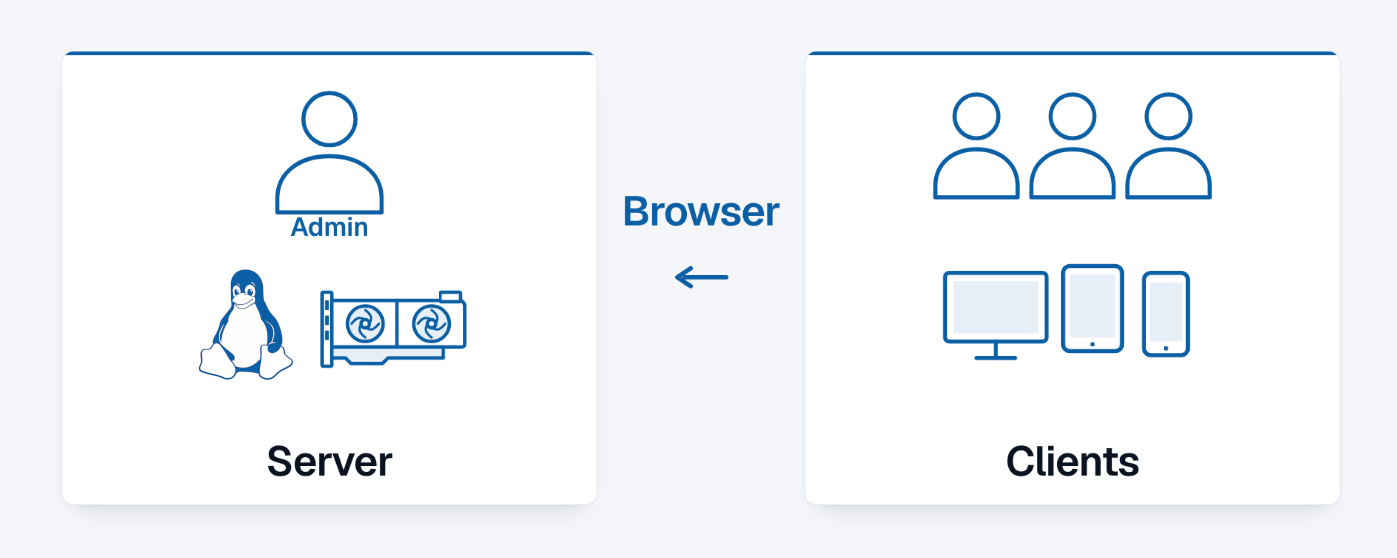
\includegraphics[width=12cm]{figures/portal_architecture.png}
  \caption{Portal Server \& many clients}
\end{figure}


\includegraphics[width=0.5cm]{../../data/icons/hint.png} Please \textbf{note} that COMPASS Portal will be a separate project with its own documentation and deployment. It is not part of the COMPASS Client. This chapter only summarizes its capabilities; for installation, deployment, configuration and detailed usage, please refer to the COMPASS Portal project documentation. \\

\begin{figure}[H]
    \centering
    \hspace*{-2.5cm}
    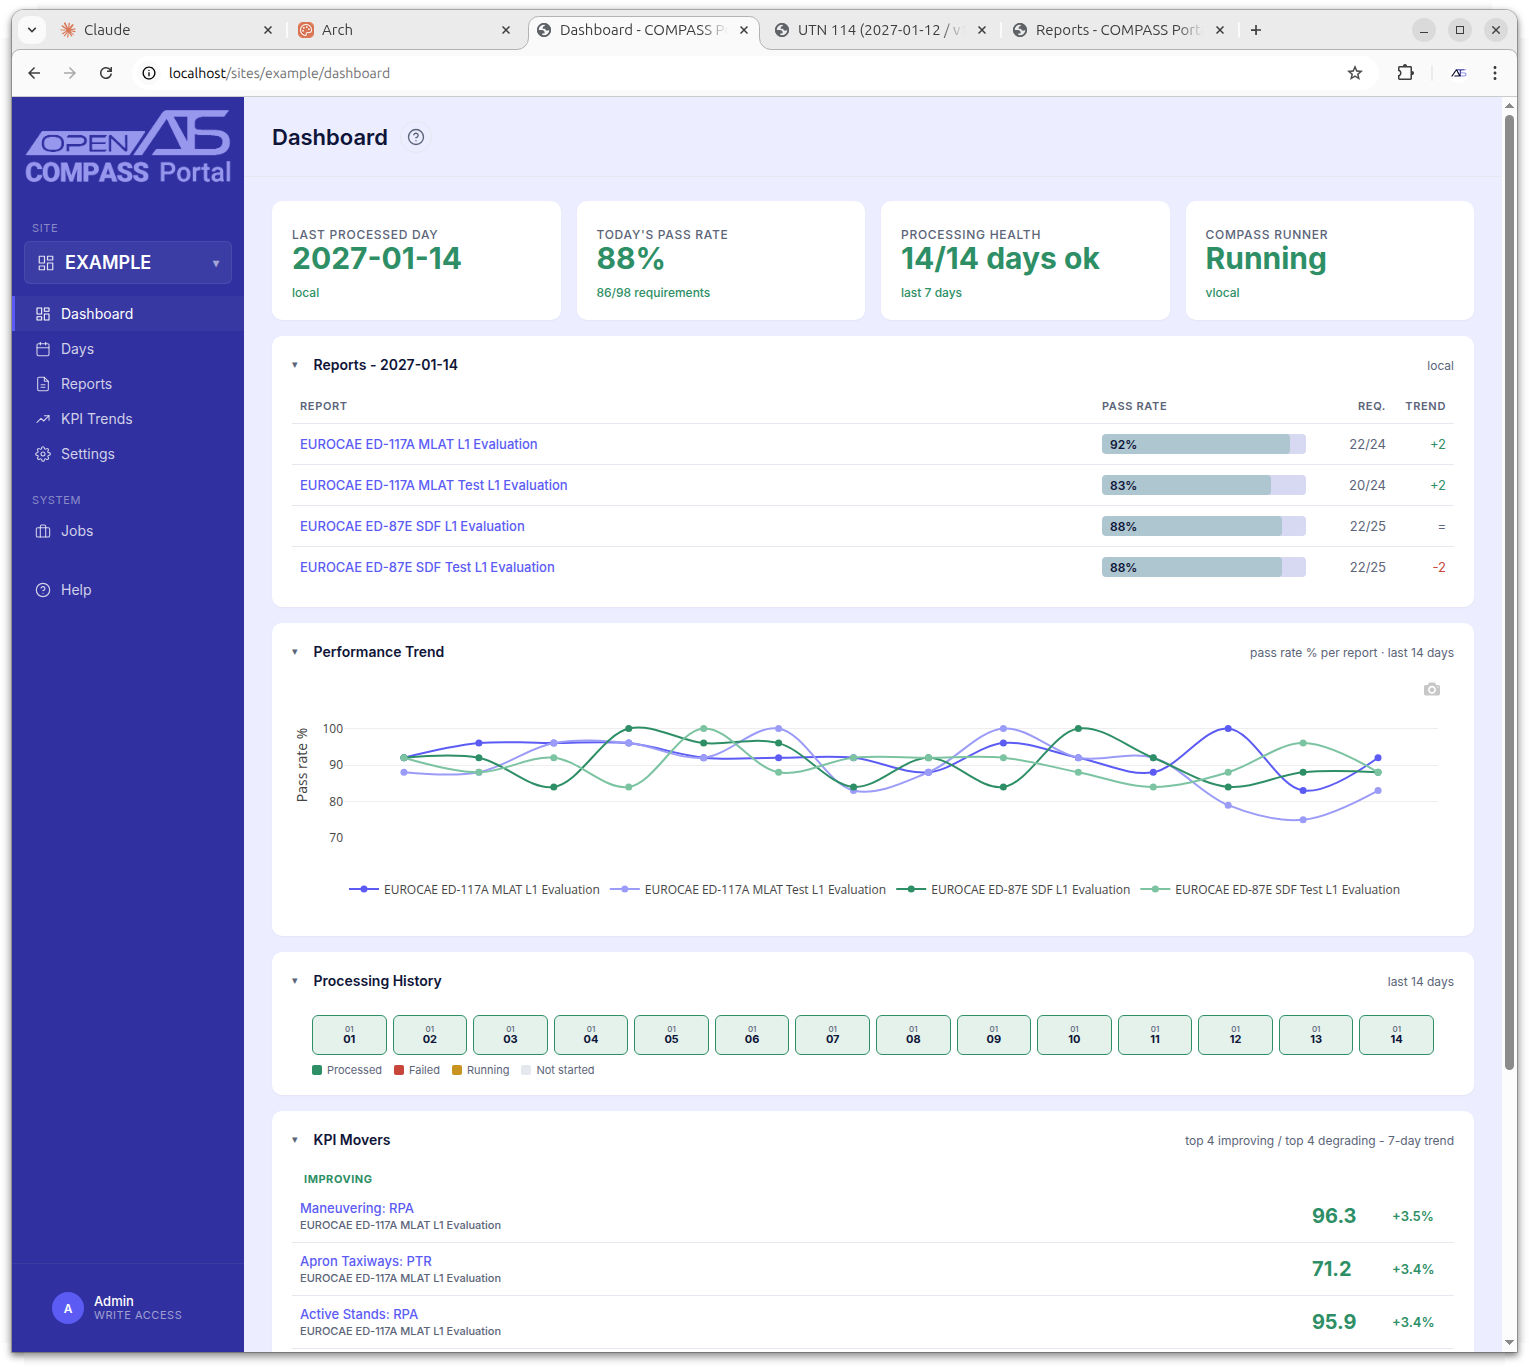
\includegraphics[width=19cm]{figures/portal_overview.png}
  \caption{Portal overview}
\end{figure}


\section{Feature Summary}

The following capabilities are provided:
\begin{itemize}
\item Job Orchestration: queued, running, finished, failed and cancelled states for ASTERIX import, reconstruction, evaluation, analyze and report export, with one COMPASS job at a time and live progress
\item Per-Day Database: self-contained DuckDB file per processed day produced by COMPASS, immutable once finalized, read directly by the Portal
\item Days, Targets and Reports: browse the rolling archive with day summaries, target search by callsign, Mode S and Mode 3/A, per-target trajectories on OpenStreetMap tiles, and a report viewer for PDF and DOCX exports including tables, figures and geographic annotations
\item Pre-configured Evaluations: define an evaluation once (reference data, test data, standard, sector layers) and apply it to every processed day with no further configuration
\item KPI Trends: configurable extraction of metrics from report tables into per-data-series history, with cascading-filter dashboard, threshold lines, pass/fail markers and per-report summaries
\item Multi-Site: one deployment hosts several independent operator contexts, each with its own archive, indices, evaluations and KPI history; a single shared backend process
\item Integration API: the same JSON endpoints serve the browser frontend and external clients, with auto-generated OpenAPI specification for 3rd-party integration
\end{itemize}
\ \\

Typical use cases include intranet-wide browsing of processed recordings and reports, scheduled nightly processing of new ASTERIX recordings, long-term KPI tracking of sensor and tracker performance, compliance trend reviews across days, weeks and months, and 3rd-party integration of analysis results via the JSON API. \\

\begin{figure}[H]
    \centering
    \hspace*{-2.5cm}
    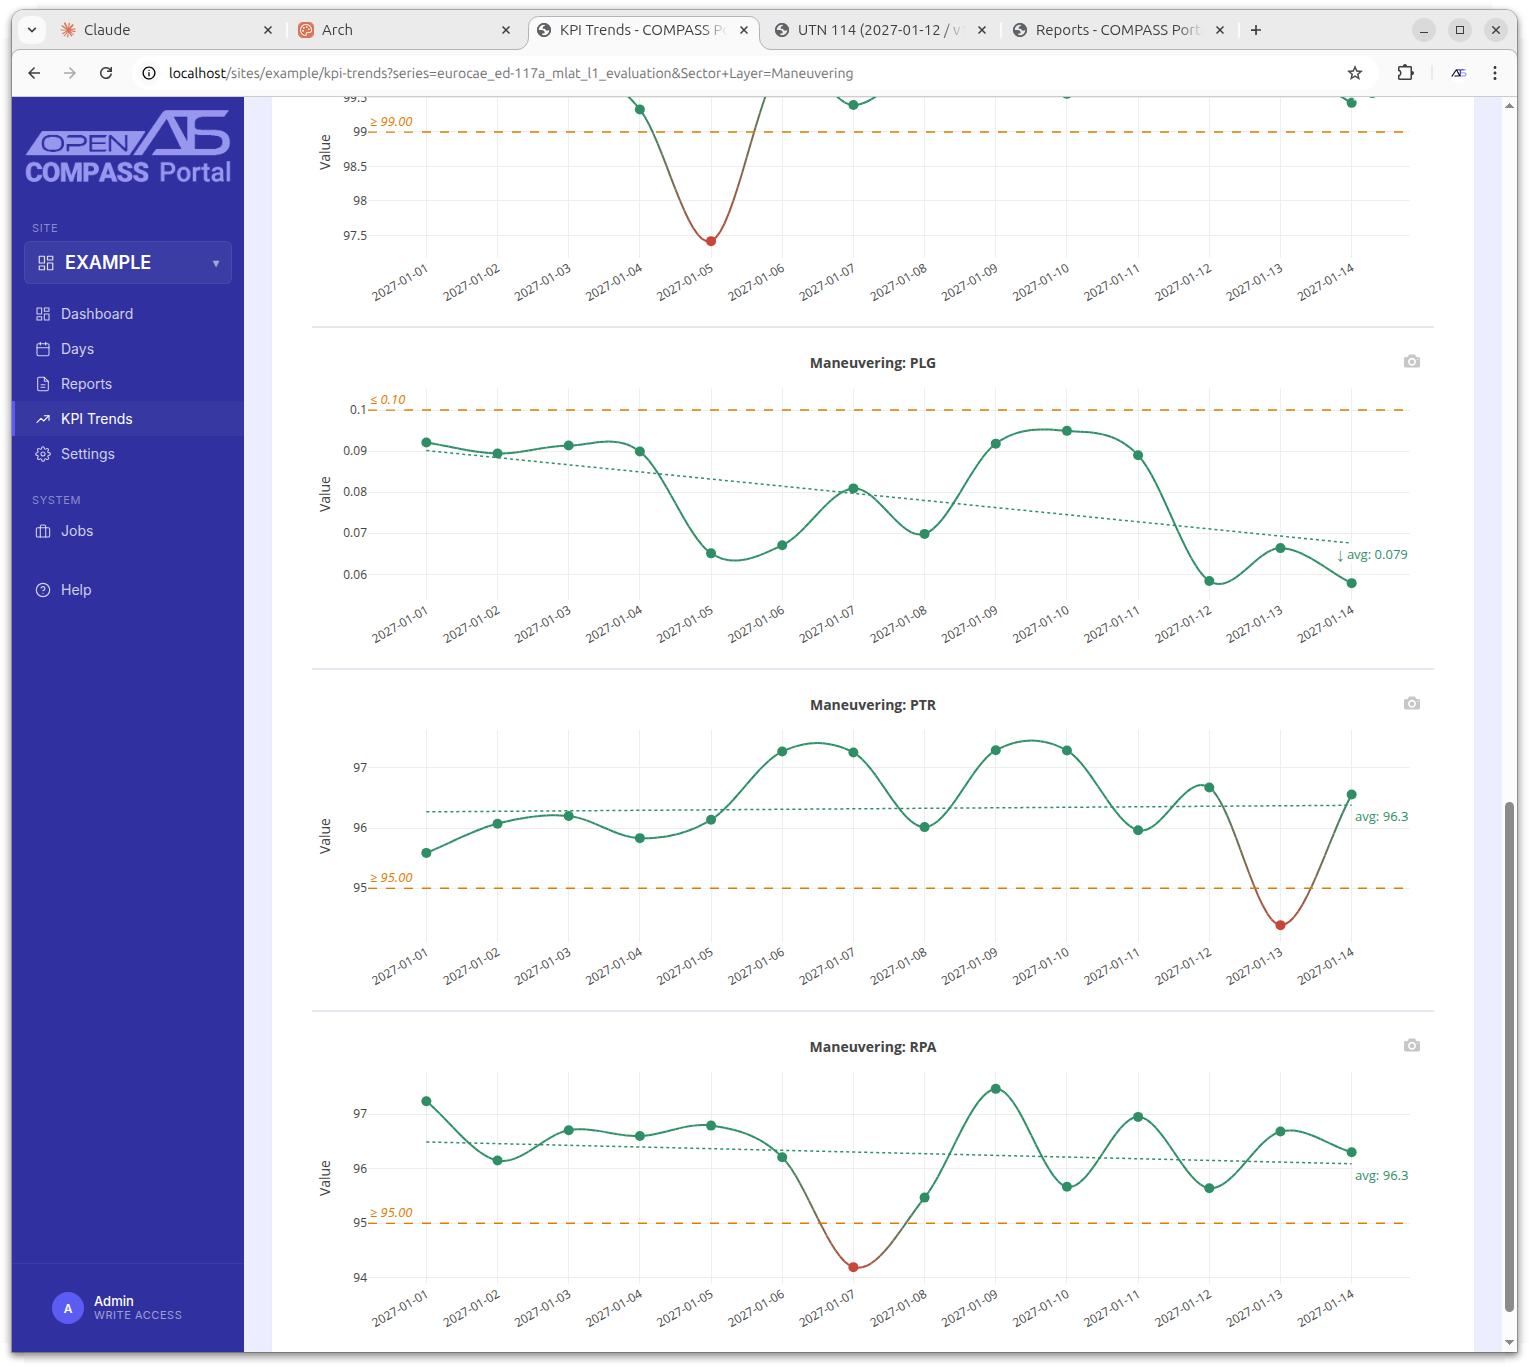
\includegraphics[width=19cm]{figures/portal_trends.png}
  \caption{Portal trends}
\end{figure}

\section{Integration with COMPASS}

COMPASS Portal does not read data through a running COMPASS Client process. Finalized per-day databases are opened directly by the Portal middleware. For tasks that require a COMPASS process (configuration, import, reconstruction, evaluation, analyze, export), job execution is delegated to a host-side runner that owns one COMPASS instance and forwards commands to it through the Runtime Command Interface (see \nameref{sec:rtcommand_interface}). \\

At any time, at most one COMPASS process is active per host, and runtime commands are serialized through the runner.

\section{Distribution and Further Documentation}

COMPASS Portal will commonly be usable in an Docker stack for a single Linux workstation. While its pricing and licensing is still to be defined, it will very likely require the professional license. \\


